\subsection{Wirksamkeit von Shift-Left Maßnahmen}

In den vorherigen Textabschnitten wurde erklärt, wie Shift-Left in unterschiedlichen Ebenen eines Projekts mit verschiedenen Tools genutzt werden kann. Um eine Einschätzung der Wirksamkeit von Shift-Left zu erhalten, wird im Folgenden ein Beitrag von \citet{andriadi_impact_2023} betrachtet.

\begin{figure}
\centering
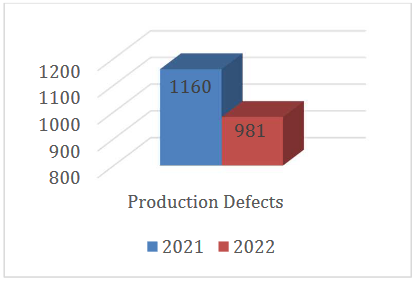
\includegraphics[width=0.9\linewidth]{images/Impact_production_defects.png}
\caption{Diagramm zur Menge an Fehlern im Jahr 2021 und 2022 \cite{andriadi_impact_2023}}
\label{fig:production_defects }
\end{figure}

\citet{andriadi_impact_2023} untersuchten dafür die Menge an Fehlern in einem indonesischen Tech-Unternehmen in den Jahren 2021 und 2022. Das Unternehmen entwickelte an einem Projekt zunächst ein Jahr ohne den Shift-Left-Ansatz und im darauffolgenden Jahr mit dem Shift-Left-Ansatz. Die Änderungen, die das Unternehmen 2022 vornahm, beinhalteten hauptsächlich die Arbeitsweise und die Rolle der Entwickler sowie der QA-Teams:
\begin{enumerate}
\item Tests werden bereits in der Entwicklungsphase geschrieben und nicht nur in einer gesonderten Testphase.
\item Entwickler schreiben Basis-Tests für ihre eigenen Features und beheben dadurch entdeckte Fehler eigenständig.
\item QA erstellt parallel automatisierte Testskripte für den aktuellen Sprint. Die Menge der manuellen Tests wurde reduziert und mehr automatisierte Tests zu schreiben.
\item Entwickler und QA halten gemeinsam tägliche Meetings, um Testanforderungen zu klären. Alle gefundenen Fehler werden dokumentiert und kategorisiert.
\end{enumerate}

Nach den zwei Jahren Entwicklung wurde die Menge an gefundenen Fehlern in beiden Jahren verglichen und überprüft ob eine Verringerung stattgefunden hat. In Abbildung \ref{fig:production_defects } ist die Menge der Produktionsfehler in beiden Jahren zu erkennen. Dabei ist festzustellen, dass die Menge an gefundenen Fehlern von 1160 auf 981 gesunken ist. Dies entspricht einer Reduzierung von etwa 15\%. Diese Verbesserung wird durch die frühere Erkennung von Fehlern in den zeitigen Entwicklungsphase begründet, da das Projekt dort weniger Quellcode und eine geringere Komplexität aufweist \cite{andriadi_impact_2023}. Ebenfalls konnten die Fehler bei Regressionstests um 24\% und bei Integrationstests um 57\% reduziert werden. Des Weiteren wurde die Anzahl an Hotfixes von 43 auf 25 verringert, was einer Reduzierung von 42\% entspricht. Alle diese Metriken zeigen, dass der genutzte Shift-Left-Ansatz dazu beigetragen hat, die Softwarequalität zu steigern und spätere Kosten zu reduzieren. \citet{andriadi_impact_2023} stellten in diesen Zuge fest, das der Prozess jedoch auch Herausforderungen mit sich bringt: Die Entwickler benötigten mehr Zeit, da sie zusätzlich Tests schreiben mussten, und der Entwicklungsprozess war abhängig von einer gut funktionierenden Kommunikation aller Beteiligten \cite{andriadi_impact_2023}. Diese Feststellung zeigt, dass der Shift-Left-Ansatz effektiv ist, gleichzeitig aber gut geplant und richtig umgesetzt werden muss.

Die in der Studie demonstrierte Wirksamkeit von Shift-Left Testing lässt sich analog auf Shift-Left-Security übertragen. Indem Sicherheitsprüfungen bereits in den frühen Entwicklungsphasen integriert werden, lassen sich Risiken minimieren und somit Kosten senken. Die vorgestellte Studie unterstützt dies indirekt, da sie zeigt, dass durch frühzeitige Qualitätssicherung kritische Defekte verhindert werden können – ein Prinzip, das sich auf Sicherheitskontexte übertragen lässt.